\documentclass[a4paper,UTF8]{article}
\usepackage{ctex}
\usepackage[margin=1.25in]{geometry}
\usepackage{color}
\usepackage{graphicx}
\usepackage{amssymb}
\usepackage{amsmath}
\usepackage{amsthm}
\usepackage{bm}
\usepackage{hyperref}
\numberwithin{equation}{section}
%\usepackage[thmmarks, amsmath, thref]{ntheorem}
\theoremstyle{definition}
\newtheorem*{solution}{Solution}
\newtheorem*{prove}{Proof}
\usepackage{multirow}

\renewcommand\refname{Reference}
\renewcommand\figurename{Figure}

%--

%--
\begin{document}
\title{机器学习导论\\
习题三}
\author{141242006, 袁帅, 141242006@smail.nju.edu.cn}
\maketitle
\section{[30pts] Decision Tree Analysis}
决策树是一类常见的机器学习方法,但是在训练过程中会遇到一些问题。

(1) \textbf{[15pts]} 试证明对于不含冲突数据(即特征向量完全相同但标记不同)的训练集,必存在与训练集一致(即训练误差为0)的决策树;

(2) \textbf{[15pts]} 试分析使用“最小训练误差”作为决策树划分选择的缺陷。
\begin{solution}
\item[(1)] For all training sets(without contradictory samples) with $n$ samples, we can prove that there must exist one decision tree corresponding to this dataset with 0 training errors, by mathematical induction as follow:
\begin{prove} 
\textbf{Basis:} When $n=1$, such decision tree could obviously be built by simply adding one node.

\textbf{Induction Hypothesis:} When $n\geq 2$, suppose the statement holds for all $1\leq k<n$.

\textbf{Induction Steps:} Consider training sets $D=(\bm{X}, \bm{y})$ with $n$ samples($n\geq 2$). We can choose a feature for split by finding such feature $a$ on which the samples take more than one value (i.e., $\exists \bm{x}_1, \bm{x}_2 \in \bm{X}$, s.t. $\bm{x}_1^{(a)}\neq\bm{x}_2^{(a)}$, where $\bm{x}^{(a)}$ denotes the value of $\bm{x}$ on feature $a$). Note that if such $a$ doesn't exist, all samples in the training sets are identical, yielding a trivial case.

Now we split the dataset $D$ by feature $a$ into $p$ sub-datasets $D_1, D_2, ..., D_p$, the number of samples of which are $n_1, n_2, ..., n_p$, respectively. Because $1\leq n_i<n$ for all $1\leq i\leq p$, according to the induction hypothesis, all these sub-datasets must have their own corresponding decision trees, and therefore by linking those trees under one single node, we generate a decision tree, which takes $a$ as the first split, for dataset $D$.
\qed
\end{prove}

\item[(2)] If we split the tree by minimizing training error, the model would suffer from overfitting. If all splits are based on training error, it does not generalize well with other data.

\end{solution}

\section{[30pts] Training a Decision Tree}
考虑下面的训练集:共计6个训练样本,每个训练样本有三个维度的特征属性和标记信息。详细信息如表\ref{table:training}所示。

请通过训练集中的数据训练一棵决策树,要求通过“信息增益”(information gain)为准则来选择划分属性。请参考书中图4.4,给出详细的计算过程并画出最终的决策树。
\begin{table}[h]
\centering
\caption{训练集信息}
\label{table:training}\vspace{2mm} 
\begin{tabular}{c|c c c|c}\hline
序号		&  特征 \textbf{A} 	&	特征 \textbf{B}	&	特征 \textbf{C} 	&	标记    \\ \hline
1		&  0 	&	1	&	1 	&	0    \\
2		&  1 	&	1 	&	1 	&	0    \\
3		&  0 	&	0 	&	0 	&	0    \\
4		&  1 	&	1 	&	0 	&	1    \\
5		&  0 	&	1 	&	0 	&	1    \\
6		&  1 	&	0 	&	1 	&	1    \\\hline
\end{tabular} 
\end{table}

\begin{solution}
We train the decision tree, split by information gain $\text{Gain}(D,a)$.

\textbf{(1)} For training set $D$ and feature set $F=\{A,B,C\}$, $|\mathcal{Y}|=2$, $p_0=\frac{1}{2}$, $p_1=\frac{1}{2}$, and therefore information entrophy $\text{Ent}(D)=-\sum_{k=0}^1p_k\log_2p_k=1$.

If $D$ is split by feature $A$, the resulting subsets $D^0=\{1,3,5\}$, $D^1=\{2,4,6\}$, $\text{Ent}(D^0)=-\frac{2}{3}\log_2\frac{2}{3}-\frac{1}{3}\log_2\frac{1}{3}=0.9183$, $\text{Ent}(D^1)=-\frac{1}{3}\log_2\frac{1}{3}-\frac{2}{3}\log_2\frac{2}{3}=0.9183$, so the information gain $\text{Gain}(D,A)=\text{Ent}(D)-\sum_{k=0}^1\frac{|D^{k}|}{|D|}\text{Ent}(D^{k})=1-0.9183=0.0817$.

If $D$ is split by feature $B$, the resulting subsets $D^0=\{3,6\}$, $D^1=\{1,2,4,5\}$, $\text{Ent}(D^0)=-\frac{1}{2}\log_2\frac{1}{2}-\frac{1}{2}\log_2\frac{1}{2}=1$, $\text{Ent}(D^1)=-\frac{1}{2}\log_2\frac{1}{2}-\frac{1}{2}\log_2\frac{1}{2}=1$, so the information gain $\text{Gain}(D,A)=\text{Ent}(D)-\sum_{k=0}^1\frac{|D^{k}|}{|D|}\text{Ent}(D^{k})=1-1=0$.

If $D$ is split by feature $C$, the resulting subsets $D^0=\{3,4,5\}$, $D^1=\{1,2,6\}$, $\text{Ent}(D^0)=-\frac{1}{3}\log_2\frac{1}{3}-\frac{2}{3}\log_2\frac{2}{3}=0.9183$, $\text{Ent}(D^1)=-\frac{2}{3}\log_2\frac{2}{3}-\frac{1}{3}\log_2\frac{1}{3}=0.9183$, so the information gain $\text{Gain}(D,A)=\text{Ent}(D)-\sum_{k=0}^1\frac{|D^{k}|}{|D|}\text{Ent}(D^{k})=1-0.9183=0.0817$.

So we will split $D$ by feature $A$, yielding $D_1=\{1,3,5\}$ and $D_2=\{2,4,6\}$.

\textbf{(2)} For $D_1=\{1,3,5\}$ and $F_1=\{B,C\}$, $|\mathcal{Y}|=2$, $p_0=\frac{2}{3}$, $p_1=\frac{1}{3}$, and therefore information entrophy $\text{Ent}(D_1)=-\sum_{k=0}^1p_k\log_2p_k=0.9183$.

If $D_1$ is split by feature $B$, the resulting subsets $D_1^0=\{3\}$, $D_1^1=\{1,5\}$, $\text{Ent}(D_1^0)=0$, $\text{Ent}(D_1^1)=-\frac{1}{2}\log_2\frac{1}{2}-\frac{1}{2}\log_2\frac{1}{2}=1$, so the information gain $\text{Gain}(D_1,B)=\text{Ent}(D_1)-\sum_{k=0}^1\frac{|D_1^{k}|}{|D_1|}\text{Ent}(D_1^{k})=0.9183-0.6667=0.2516$.

If $D_1$ is split by feature $C$, the resulting subsets $D_1^0=\{3,5\}$, $D_1^1=\{1\}$, $\text{Ent}(D_1^0)=-\frac{1}{2}\log_2\frac{1}{2}-\frac{1}{2}\log_2\frac{1}{2}=1$, $\text{Ent}(D_1^1)=0$, so the information gain $\text{Gain}(D_1,C)=\text{Ent}(D_1)-\sum_{k=0}^1\frac{|D_1^{k}|}{|D_1|}\text{Ent}(D_1^{k})=0.9183-0.6667=0.2516$.

So we will split $D_1$ by feature $B$, yielding $D_3=\{3\}$ and $D_4=\{1,5\}$.

\textbf{(3)} For $D_2=\{2,4,6\}$ and $F_2=\{B,C\}$, $|\mathcal{Y}|=2$, $p_0=\frac{1}{3}$, $p_1=\frac{2}{3}$, and therefore information entrophy $\text{Ent}(D_1)=-\sum_{k=0}^1p_k\log_2p_k=0.9183$.

If $D_2$ is split by feature $B$, the resulting subsets $D_2^0=\{6\}$, $D_2^1=\{2,4\}$, $\text{Ent}(D_2^0)=0$, $\text{Ent}(D_2^1)=-\frac{1}{2}\log_2\frac{1}{2}-\frac{1}{2}\log_2\frac{1}{2}=1$, so the information gain $\text{Gain}(D_2,B)=\text{Ent}(D_2)-\sum_{k=0}^1\frac{|D_2^{k}|}{|D_2|}\text{Ent}(D_2^{k})=0.9183-0.6667=0.2516$.

If $D_2$ is split by feature $C$, the resulting subsets $D_2^0=\{4\}$, $D_2^1=\{2,6\}$, $\text{Ent}(D_2^0)=0$, $\text{Ent}(D_2^1)=-\frac{1}{2}\log_2\frac{1}{2}-\frac{1}{2}\log_2\frac{1}{2}=1$, so the information gain $\text{Gain}(D_2, C)=\text{Ent}(D_2)-\sum_{k=0}^1\frac{|D_2^{k}|}{|D_2|}\text{Ent}(D_2^{k})=0.9183-0.6667=0.2516$.

So we will split $D_2$ by feature $B$, yielding $D_5=\{6\}$ and $D_6=\{2,4\}$.

\textbf{(4)} For $D_4=\{1,5\}$ and $F_4=\{C\}$, the last split would by feature $C$.

\textbf{(5)} For $D_6=\{2,4\}$ and $F_6=\{C\}$, the last split would by feature $C$.

Therefore, the consequent decision tree could be shown as below:
\begin{figure}[htbp] %  figure placement: here, top, bottom, or page
   \centering
   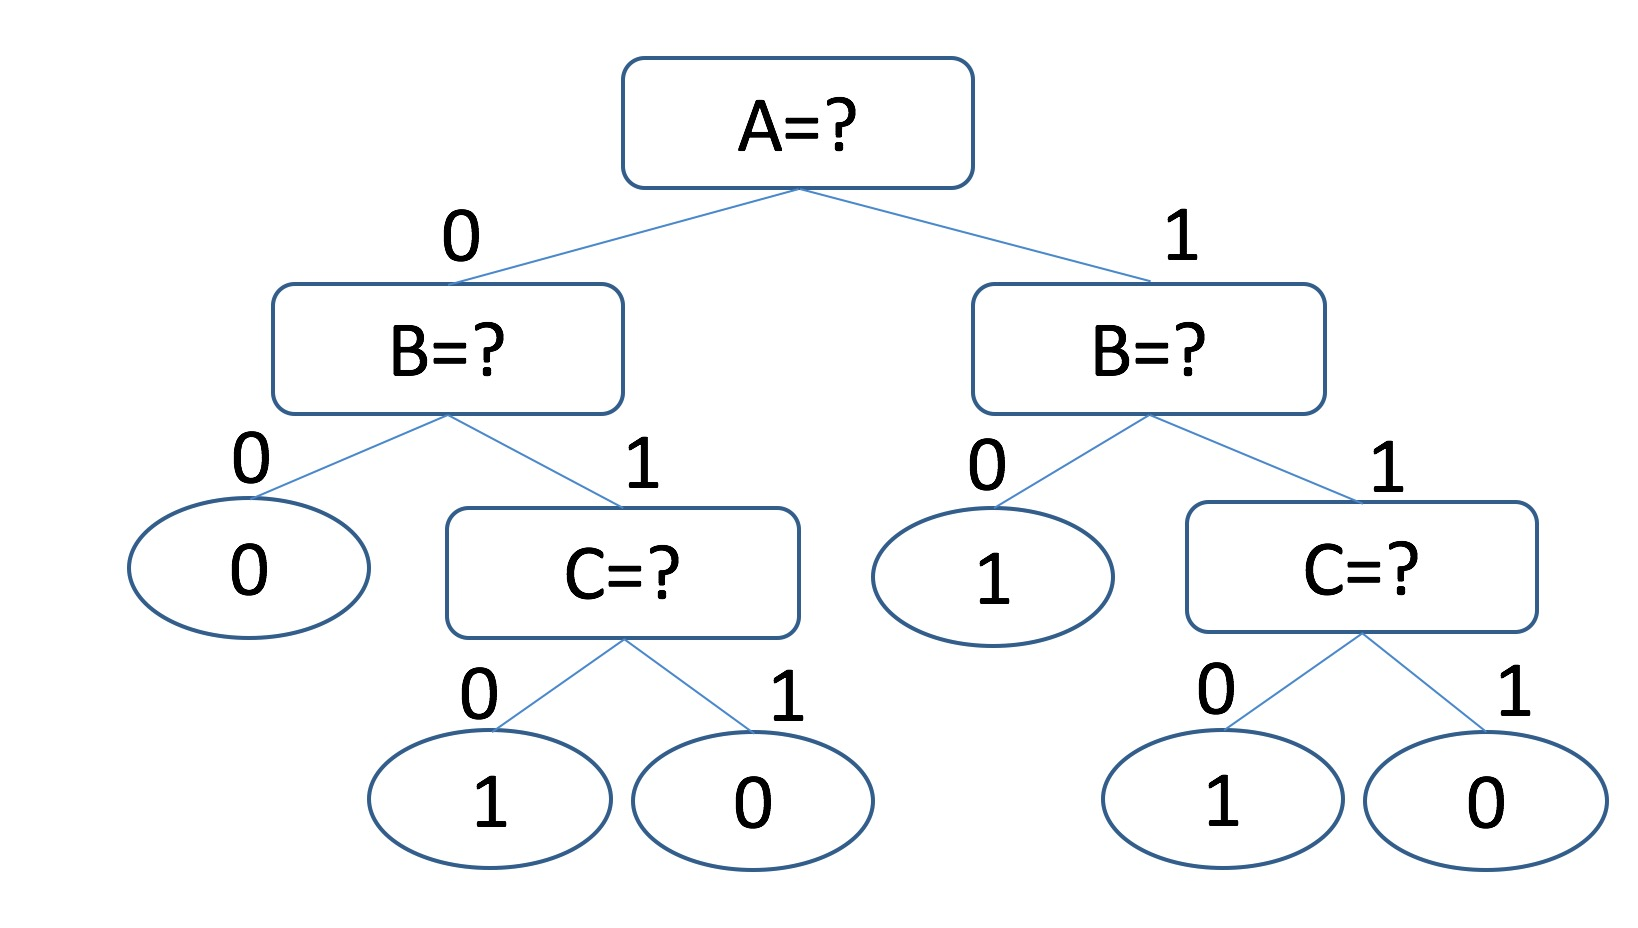
\includegraphics[width=4in]{decisionTree.png} 
   \caption{Decision tree for training set $D$}
   \label{fig:example}
\end{figure}

\end{solution}

\section{[40pts] Back Propagation} 
单隐层前馈神经网络的误差逆传播(error BackPropagation,简称BP)算法是实际工程实践中非常重要的基础,也是理解神经网络的关键。

请编程实现BP算法,算法流程如课本图5.8所示。详细编程题指南请参见链接:\url{http://lamda.nju.edu.cn/ml2017/PS3/ML3_programming.html}

在实现之后,你对BP算法有什么新的认识吗?请简要谈谈。
\begin{solution}
I implemented the code in MATLAB, yielding an accuracy around 94\%. The core thing of BP neural networks is nothing but a gradient descent approach, in which the gradient could be vividly calculated and presented.
\end{solution}

\section*{附加题   [30pts] Neural Network in Practice}
在实际工程实现中,通常我们会使用已有的开源库,这样会减少搭建原有模块的时间。因此,请使用现有神经网络库,编程实现更复杂的神经网络。详细编程题指南请参见链接:\url{http://lamda.nju.edu.cn/ml2017/PS3/ML3_programming.html}

和上一题相比,模型性能有变化吗?如果有,你认为可能是什么原因。同时,在实践过程中你遇到了什么问题,是如何解决的?
\begin{solution}
With the help of Keras Documentation\cite{ref: doc}, I finished the code in Python. The model training process is much faster than the previous model, while no significant progress is found in accuracy. The training speed increases a lot because of the proper implementation and compiling optimization of library functions; the accuracy is not improved because our previous code already works well enough: 94\% accuracy is arguably high for a MNIST dataset with only 3000 training samples.
~\\
\end{solution}

\begin{thebibliography}{99}
\bibitem{ref: doc}\textit{Keras Documentation}. \url{https://keras.io/optimizers/}.
\end{thebibliography}

\end{document}